\documentclass{article}
\usepackage[utf8]{inputenc}
\usepackage[margin=1in]{geometry}
\usepackage{amsmath,graphicx,amsfonts}

\title{EECS445 Project 1}
\author{Dong Zhengyuan (dongzy)}
\date{February 10, 2019}
\graphicspath{{images/}}

\usepackage{listings}
\usepackage{color}

\definecolor{dkgreen}{rgb}{0,0.6,0}
\definecolor{gray}{rgb}{0.5,0.5,0.5}
\definecolor{mauve}{rgb}{0.58,0,0.82}

\lstset{frame=tb,
  language=Python,
  aboveskip=3mm,
  belowskip=3mm,
  showstringspaces=false,
  columns=flexible,
  basicstyle={\small\ttfamily},
  numbers=none,
  numberstyle=\tiny\color{gray},
  keywordstyle=\color{blue},
  commentstyle=\color{dkgreen},
  stringstyle=\color{mauve},
  breaklines=true,
  breakatwhitespace=true,
  tabsize=3
}

\begin{document}

\maketitle

\section*{2 Feature Extraction}
\textbf{(c)}
The number of unique words is 2850,
The number of average non-zero features is 15.624

\section*{3 Hyperparameter Feature Selection}
\subsection*{3.1 Hyperparameter Selection for a Linear-Kernel SVM}
\textbf{(a)} In an iteration of cross-validation, we take one fold as the validtion set and
the rest folds as the training set. Therefore, if we maintain class proportiions across folds,
we will have a balanced training set in each iteration of the cross-validation
and do not need to compensate for class imbalances.\\ \\
\textbf{(c)} The optimal parameter under different metrics is shown below: \\ \\
\begin{tabular}{|c|c|c|}
\hline
\bf Performance Metric & \bf C & \bf Performance \\ \hline
Accuracy & 0.1 & 0.839 \\ \hline
F1-Score & 0.1 & 0.838 \\ \hline
AUROC & 0.1 & 0.920 \\ \hline
Precision & 10 & 0.841 \\ \hline
Sensitivity & 0.001 & 0.864 \\ \hline
Specificity & 10 & 0.844 \\ \hline
\end{tabular}\\ \\
\indent Generally, as C increases, CV performance increases to the peak,
then gently decreases. This trend is shared among metrics,
except for sensitivity, where the peak is reached at the beginning when $C=0.001$. \\
\indent If I have to train a final model, I will optimize for accuracy
when choosing $C$, since the recognition of both positive and negative classes
are important, and accuracy is the most direct metric to address that importance.\\ \\
\textbf{(d)} Using $C=0.1$ which maximizes accuracy, the performance of the SVM under different metrics is shown below: \\ \\
\begin{tabular}{|c|c|c|}
\hline
\bf Performance Metric & \bf Performance \\ \hline
Accuracy &  0.833 \\ \hline
F1-Score &  0.830 \\ \hline
AUROC &  0.921 \\ \hline
Precision &  0.845 \\ \hline
Sensitivity &  0.815 \\ \hline
Specificity &  0.850 \\ \hline
\end{tabular}\\ \\ \\
\textbf{(e)} The plot is shown below:\\
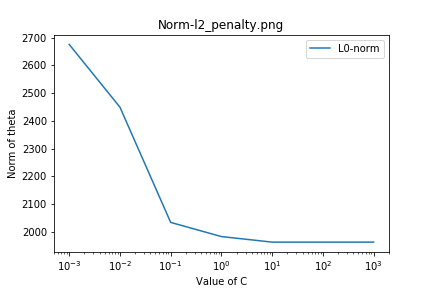
\includegraphics[width=.5\textwidth]{31e.png}\\
\indent We can see that the L0-norm of $\bar{\theta}$ decreases as $C$ increases,
but gradually converges to 2000.\\ \\
\textbf{(f)} The most positive / negative words are shown below:\\ \\
\begin{tabular}{|c|c||c|c|}
\hline
\bf Positive Coefficient & \bf Word & \bf Negative Coefficent & \bf Word\\ \hline
0.969 & thanks & -0.615 & hours \\ \hline
0.901 & thank & -0.549 & delayed \\ \hline
0.765 & great & -0.521 & due \\ \hline
0.596 & good & -0.507 & good \\ \hline
\end{tabular}\\ \\
\subsection*{3.2 Hyperparameter Selection for a Quadratic-Kernel SVM}
\textbf{(a)} The optimal parameters under different metrics are shown below:\\ Grid search: \\\\
\begin{tabular}{|c|c|c|c|}
\hline
\bf Performance Metric & \bf C & \bf r & \bf Performance \\ \hline
Accuracy & 10 & 1000 & 0.840 \\ \hline
F1-Score & 10 & 1000 & 0.839 \\ \hline
AUROC & 1000 & 0.1 & 0.918 \\ \hline
Precision & 10 & 1000 & 0.846 \\ \hline
Sensitivity & 0.001 & 0.001 & 0.948 \\ \hline
Specificity & 10 & 100 & 0.848 \\ \hline
\end{tabular}\\ \\
Random search: \\\\
\begin{tabular}{|c|c|c|c|}
\hline
\bf Performance Metric & \bf C & \bf r & \bf Performance \\ \hline
Accuracy & 136.61 & 5.077 & 0.848 \\ \hline
F1-Score & 136.61 & 5.077 & 0.846 \\ \hline
AUROC & 136.61 & 5.077 & 0.916 \\ \hline
Precision & 136.61 & 5.077 & 0.852 \\ \hline
Sensitivity & 0.0014 & 0.0033 & 0.918 \\ \hline
Specificity & 136.61 & 5.077 & 0.854 \\ \hline
\end{tabular}\\ \\
\textbf{(b)} The AUROC results are shown below:\\\\
\begin{tabular}{|c|c|c|c|}
\hline
\bf Tuning Scheme & \bf C & \bf r & \bf AUROC \\ \hline
Grid Search & 1000 & 0.1 & 0.918 \\ \hline
Random Search & 136.61 & 5.077 & 0.916\\ \hline
\end{tabular}\\\\
\indent Generally, for a given $C$, the performance increases as $r$ increases,
for a given $r$, the performance increases and then decreases as $C$ increases.
The use of random search is generally better than grid search,
as it visits more distinct values of $C$ and $r$.
If $C$ and $r$ do not contribute equally to CV-performance
(which is usually the case), random search is more likely to get closer to
the optimal value of the predominant hyperparameter. Random search also gives more consistent results among metrics
(5 of the 6 metrics gives the same result)
\subsection*{3.3 Learning Non-linear Classifiers with a Linear-Kernel SVM}
\textbf{(a)} The quadratic kernel is $K(\bar{x},\bar{x}')=(\bar{x}\cdot \bar{x}'+r)^2$.
Suppose $\bar{x},\bar{x}'\in \mathbb{R}^d$, we can expand it as
\begin{align*}
K(\bar{x},\bar{x}')=&(\sum_{i=1}^{d}x_ix'_i+r)^2=(\sum_{i=1}^{d}x_ix'_i)^2+2(\sum_{i=1}^{d}x_ix'_i)r+r^2 \\
=& \sum_{i=1}^d (x_ix'_i)^2+2\sum_{i=1}^{d-1}\sum_{j=i+1}^d (x_ix'_i)(x_jx'_j)+2(\sum_{i=1}^{d}x_ix'_i)r+r^2 \\
=& \sum_{i=1}^d x_i^2 x'_i^2+2\sum_{i=1}^{d-1}\sum_{j=i+1}^d (x_ix_j)(x'_ix'_j)+2r(\sum_{i=1}^{d}x_ix'_i)+r^2 \\
=& \phi(\bar{x}) \phi(\bar{x}')
\end{align*}
Therefore $\phi(x)=[(x_i^2)_{i=1..d}, (\sqrt{2}x_ix_j)_{i=1..d-1, j=i+1..d}, (\sqrt{2r}x_i)_{i=1..d}, r]^T$ \\\\
\textbf{(b)} Explicit feature mappings are more flexible and always produces a valid kernel when multiplied,
while kernel functions must satisfy Mercer's Theorem.
However, explicit feature mappings can be difficult, sometimes impossible (rbf kernel) to compute,
while kernel functions can be computed much faster.

\subsection*{3.4 Linear-Kernel SVM with L1 Penalty and Squared Hinge Loss}
\textbf{(a)} The default max\_iter=1000 is not enough for convergence, and the result is undeterministic.
Among about 10 trials, AUROC varies between 0.91 and 0.92. In most cases $C=1000$ is optimal, but sometimes $C=100$.
After modifying max\_iter to 10000, the algorithm converges, but the result is still undeterministic. \\\\
\textbf{(b)} The plot is shown below:\\
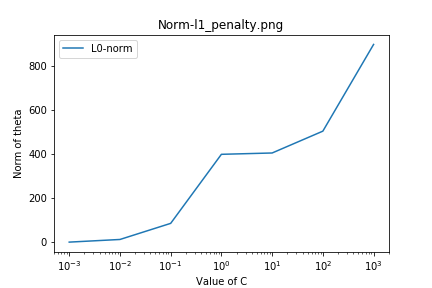
\includegraphics[width=.5\textwidth]{34b.png}\\\\
\textbf{(c)} The L1 penalty significantly decreases the L0-norm of the learned parameter.
Also, under L1 norm, the L0-norm of the learned parameter increases as $C$ increases.\\\\
\textbf{(d)} If we use Hinge Loss instead of Squared Hinge Loss, the penalty on the misclassified data points will be lighter.
More data points will become support vectors and have non-zero parameter.
Therefore, the optimal solution will have a greater L0-norm under Hinge Loss.\\
\section*{4 Asymmetric Cost Functions and Class Imbalance}
\subsection*{4.1 Arbitrary class weights}
\textbf{(a)} If $W_n$ is much greater than $W_p$, misclassified negative data points will be much more severely penalized
than misclassified positive data points. Our model will be trained to emphasize more on correctly classifying negative data points.\\\\
\textbf{(b)} The performance of the modified SVM is shown below:\\\\
\begin{tabular}{|c|c|c|}
\hline
\bf Performance Metric & \bf Performance \\ \hline
Accuracy &  0.563 \\ \hline
F1-Score &  0.222 \\ \hline
AUROC &  0.905 \\ \hline
Precision &  1.0 \\ \hline
Sensitivity &  0.125 \\ \hline
Specificity &  1.0 \\ \hline
\end{tabular}\\ \\\\
\textbf{(c)} Compared to 3.1(d), F1-score and sensitivity are affected the most.
As stated in 4.1(a), the new class weights make the model emphasize more on classifying negative data points and lowers
sensitivity, which is the metric for classifying positive data points. Since F1-score is a function of sensitivity,
it gets affected as well.
\subsection*{4.2 Imbalanced data}
\textbf{(a)} The performance of the SVM with $C=0.01$, $W_n=W_p=1$ is shown below:\\\\
\begin{tabular}{|c|c|c|}
\hline
\bf Performance Metric & \bf Performance \\ \hline
Accuracy &  0.384 \\ \hline
F1-Score &  0.374 \\ \hline
AUROC &  0.911 \\ \hline
Precision &  1.0 \\ \hline
Sensitivity &  0.23 \\ \hline
Specificity &  1.0 \\ \hline
\end{tabular}\\ \\\\
\textbf{(b)} In the imbalanced data set in this question, there are more negative points than positive points.
If we train the SVM with balanced class weights, we end up penalizing more on misclassified negative points and
make the model better at classifying negative points, as indicated by specificity=1.
However, the model performed poorly at classifying positive points, as indicated by a low sensitivity.
\subsection*{4.3 Choosing appropriate class weights}
\textbf{(a)} Since there are more negative points than positive points, metrics that evaluates the classification of both classes tend to be dominated by the majority class. The F1-score is more informative in such situation since it focuses on
classifying positive points and maintains a balance between sensitivity and precision,
which helps mitigating the situation in 4.2. \\
\indent A coarse grid search is performed first to determine a reasonable, smaller range of class weights.
After finding a smaller range, another random search is performed. Considering that in the imbalanced dataset here,
the proportion between negative and positive points is about 3:1, $W_n:W_p$ is fixed inverse-proportionally to 1:3
to further reduce the effort wasted. \\
\indent This approach gives its best results as $W_n=0.212$, $W_p=0.636$ ($C=1$),
which achieves F1-Score=0.777 in cross-validation. The corresponding test performances are shown below: \\\\
\begin{tabular}{|c|c|c|}
\hline
\bf Performance Metric & \bf Performance \\ \hline
Accuracy &  0.858 \\ \hline
F1-Score &  0.905 \\ \hline
AUROC &  0.938 \\ \hline
Precision &  0.971 \\ \hline
Sensitivity &  0.848 \\ \hline
Specificity &  0.9 \\ \hline
\end{tabular}\\ \\\\
\subsection*{4.4 The ROC curve}
\textbf{(a)} The ROC curves are shown below:\\
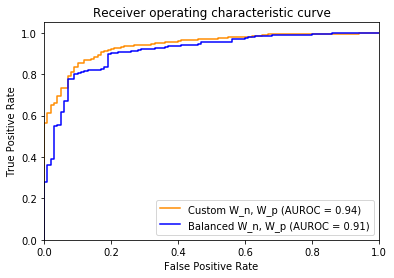
\includegraphics[width=.5\textwidth]{44.png}\\
\section*{5 Challenge}
\indent For this challenge, I attempted various approaches to train the model,
including those used in previous sections and some new approaches.
Since we have three classes and we are equally interested in identifying each one,
accuracy is a decent metric to evaluate the performance.
Since the ground truth of the test set is unknown,
I chose to optimize hyperparameters based on the accuracy score of 5-fold cross-validation.\\\\
\textbf{Approach 1: Quadratic-kernel SVC, search for $C$ and $r$}\\
\indent To start with, I used a quadratic-kernel SVC that is previously used.
I first applied a grid search within range
\{$10^{-3}$, $10^{-2}$, ..., $10^2$, $10^3$\} for both $C$ and $r$,
and the best performance 0.715 was achieved when $C=1$, $r=1000$.
Around that optimal value I conducted a second random search of 25 points,
with $\lg C \in [-1,1]$ and $\lg r \in [2,4]$ uniformly distributed.
The best performance 0.718 was achieved when $C=0.206$, $r=908.7$.\\\\
\textbf{Approach 2: Linear SVC with L1 penalty, grid search for $C$}\\
\indent The quadratic SVC hyperparameter selection was time consuming, so I switched to linear SVC with L1 penalty.
I searched $C$ within range \{$10^{-3}$, $10^{-2}$, ..., $10^2$, $10^3$\}.
The best performance 0.7076 was achieved when $C=1$.\\\\
\textbf{Approach 3: Linear SVC with L2 penalty, grid search for $C$}\\
\indent Still using a linear SVC, I switched to L2 penalty and searched for $C$
within the same range. This time, the best performance 0.726 is achieved when $C=0.1$.\\\\
\textbf{Approach 4: Finer grid search with word counting and normalization}\\
\indent The results from linear SVC with L2 penalty seems better,
so I decided to stick to that model and explore the effect of feature engineering on the results. I modified the \texttt{generate\_feature\_matrix}
and added two options: Counting the number of times a word occurs in a review
and normalizing each row of the feature matrix.
I also made a finer grid search by having 41 values evenly distributed between
$\lg C=-2$ and $\lg C=2$.
It turns out that the two feature generating options does not improve the result of the model. The four combinations of these two options being On/Off
gives the same best performance 0.731 when $C=0.040$,
the improvement mainly due to a finer grid. I think the reason it did not work
is that compared to the dictionary size,
the number of duplicate words in a comment is small,
let alone these duplicate words are often neutral words without emotional inclination
like "I", "and", "to", "at". \\\\
\textbf{Approach 5: Quadratic-kernel SVC under OvO mode}\\
\indent Finally, I investigated the difference between OvO and OvR in a quadratic kernel SVC.
In Approach 1 the \texttt{decision\_function\_shape} is set to OvR by default.
Here I changed it to OvO and searched for $C$ and $r$ within the same range as used in Approach 1.
The best performace 0.712 was achieved when $C=1$, $r=1000$,
which is not very different from the result of approach 1.\\\\
\textbf{Conclusion} After these approaches, I decided to choose a linear SVC with L2 penalty as my final model, with $C=0.040$

\newpage
\section*{Appendix: Code}
\subsection*{Functions}
\begin{lstlisting}
#!/usr/bin/env python
# EECS 445 - Winter 2018
# Project 1 - project1.py

import pandas as pd
import numpy as np
import itertools
import string
import random

from sklearn.svm import SVC, LinearSVC
from sklearn.model_selection import StratifiedKFold, GridSearchCV
from sklearn import metrics
from matplotlib import pyplot as plt

def select_classifier(penalty='l2', c=1.0, degree=1, r=0.0, class_weight='balanced'):
    """
        Return a linear svm classifier based on the given
        penalty function and regularization parameter c.
        """
    # TODO: Optionally implement this helper function if you would like to
    # instantiate your SVM classifiers in a single function. You will need
    # to use the above parameters throughout the assignment.
    if penalty=="l2":
        if degree==1:
            return SVC(kernel="linear", C=c, degree=degree, coef0=r, class_weight=class_weight)
        return SVC(kernel="poly", C=c, degree=degree, gamma="auto",coef0=r, class_weight=class_weight)
    if penalty=="l1":
        return LinearSVC(penalty="l1", C=c, class_weight=class_weight, dual=False, max_iter=10000)


def extract_dictionary(df):
    """
        Reads a panda dataframe, and returns a dictionary of distinct words
        mapping from each distinct word to its index (ordered by when it was found).
        Input:
        df: dataframe/output of load_data()
        Returns:
        a dictionary of distinct words that maps each distinct word
        to a unique index corresponding to when it was first found while
        iterating over all words in each review in the dataframe df
        """
    word_dict = {}

    # TODO: Implement this function
    index=0
    for text in df["text"]:
        for p in string.punctuation:
            text=text.replace(p," ")
        text=text.lower()
        spl=text.split()
        for word in spl:
            if word not in word_dict:
                word_dict[word]=index
                index=index+1
    return word_dict


def generate_feature_matrix(df, word_dict):
    """
        Reads a dataframe and the dictionary of unique words
        to generate a matrix of {1, 0} feature vectors for each review.
        Use the word_dict to find the correct index to set to 1 for each place
        in the feature vector. The resulting feature matrix should be of
        dimension (number of reviews, number of words).
        Input:
        df: dataframe that has the ratings and labels
        word_list: dictionary of words mapping to indices
        Returns:
        a feature matrix of dimension (number of reviews, number of words)
        """
    number_of_reviews = df.shape[0]
    number_of_words = len(word_dict)
    feature_matrix = np.zeros((number_of_reviews, number_of_words))
    # TODO: Implement this function
    index=0
    for text in df["text"]:
        for p in string.punctuation:
            text=text.replace(p," ")
        text=text.lower()
        spl=text.split()
        for word in spl:
            if word in word_dict:
                feature_matrix[index,word_dict[word]]=1
        index=index+1
    return feature_matrix

def cv_performance(clf, X, y, k=5, metric="accuracy"):
    """
        Splits the data X and the labels y into k-folds and runs k-fold
        cross-validation: for each fold i in 1...k, trains a classifier on
        all the data except the ith fold, and tests on the ith fold.
        Calculates the k-fold cross-validation performance metric for classifier
        clf by averaging the performance across folds.
        Input:
        clf: an instance of SVC()
        X: (n,d) array of feature vectors, where n is the number of examples
        and d is the number of features
        y: (n,) array of binary labels {1,-1}
        k: an int specifying the number of folds (default=5)
        metric: string specifying the performance metric (default='accuracy'
        other options: 'f1-score', 'auroc', 'precision', 'sensitivity',
        and 'specificity')
        Returns:
        average 'test' performance across the k folds as np.float64
        """
    # TODO: Implement this function
    scores = []
    #HINT: You may find the StratifiedKFold from sklearn.model_selection
    #to be useful
    skf = StratifiedKFold(n_splits=k)
    skf.get_n_splits(X,y)
    for train_index, test_index in skf.split(X, y):
        X_train, X_test = X[train_index], X[test_index]
        y_train, y_test = y[train_index], y[test_index]
        clf.fit(X_train,y_train)
        y_pred = clf.predict(X_test)
        if metric=="auroc":
            y_pred=clf.decision_function(X_test)
        score=performance(y_test, y_pred, metric)
        scores.append(score)

    #And return the average performance across all fold splits.
    return np.array(scores).mean()


def select_param_linear(X, y, k=5, metric="accuracy", C_range = [], penalty='l2'):
    """
        Sweeps different settings for the hyperparameter of a linear-kernel SVM,
        calculating the k-fold CV performance for each setting on X, y.
        Input:
        X: (n,d) array of feature vectors, where n is the number of examples
        and d is the number of features
        y: (n,) array of binary labels {1,-1}
        k: int specifying the number of folds (default=5)
        metric: string specifying the performance metric (default='accuracy',
        other options: 'f1-score', 'auroc', 'precision', 'sensitivity',
        and 'specificity')
        C_range: an array with C values to be searched over
        Returns:
        The parameter value for a linear-kernel SVM that maximizes the
        average 5-fold CV performance.
        """
    # TODO: Implement this function
    #HINT: You should be using your cv_performance function here
    #to evaluate the performance of each SVM
    maxc=0
    maxperf=0
    for c in C_range:
        clf = select_classifier(c=c)
        perf = cv_performance(clf, X, y, k=5, metric=metric)
        print(c, perf)
        if perf>maxperf:
            maxperf=perf
            maxc=c
    return maxc


def plot_weight(X,y,penalty,metric="",C_range=[]):
    """
        Takes as input the training data X and labels y and plots the L0-norm
        (number of nonzero elements) of the coefficients learned by a classifier
        as a function of the C-values of the classifier.
        """

    print("Plotting the number of nonzero entries of the parameter vector as a function of C")
    norm0 = []

    # TODO: Implement this part of the function
    #Here, for each value of c in C_range, you should
    #append to norm0 the L0-norm of the theta vector that is learned
    #when fitting an L2- or L1-penalty, degree=1 SVM to the data (X, y)

    for c in C_range:
        clf = select_classifier(penalty=penalty, c=c)
        clf.fit(X,y)
        n0=0
        for theta in clf.coef_:
            for c in theta:
                if c!=0:
                    n0+=1
        norm0.append(n0)

    #This code will plot your L0-norm as a function of c
    plt.plot(C_range, norm0)
    plt.xscale('log')
    plt.legend(['L0-norm'])
    plt.xlabel("Value of C")
    plt.ylabel("Norm of theta")
    plt.title('Norm-'+penalty+'_penalty.png')
    plt.savefig('Norm-'+penalty+'_penalty.png')
    plt.close()


def select_param_quadratic(X, y, k=5, metric="accuracy", param_range=[]):
    """
        Sweeps different settings for the hyperparameters of an quadratic-kernel SVM,
        calculating the k-fold CV performance for each setting on X, y.
        Input:
        X: (n,d) array of feature vectors, where n is the number of examples
        and d is the number of features
        y: (n,) array of binary labels {1,-1}
        k: an int specifying the number of folds (default=5)
        metric: string specifying the performance metric (default='accuracy'
        other options: 'f1-score', 'auroc', 'precision', 'sensitivity',
        and 'specificity')
        parameter_values: a (num_param, 2)-sized array containing the
        parameter values to search over. The first column should
        represent the values for C, and the second column should
        represent the values for r. Each row of this array thus
        represents a pair of parameters to be tried together.
        Returns:
        The parameter value(s) for a quadratic-kernel SVM that maximize
        the average 5-fold CV performance
        """
    # TODO: Implement this function
    # Hint: This will be very similar to select_param_linear, except
    # the type of SVM model you are using will be different...

    maxc=0
    macr=0
    maxperf=0
    for c,r in param_range:
        clf = select_classifier(c=c, degree=2, r=r)
        #clf = SVC(kernel = 'poly', gamma = 'auto',degree = 2, C = c, coef0 = r, class_weight = 'balanced')
        perf=cv_performance(clf, X, y, k=k, metric=metric)
        print(c,r,perf)
        if perf>maxperf:
            maxc=c
            maxr=r
            maxperf=perf
    return maxc, maxr


def performance(y_true, y_pred, metric="accuracy"):
    """
        Calculates the performance metric as evaluated on the true labels
        y_true versus the predicted labels y_pred.
        Input:
        y_true: (n,) array containing known labels
        y_pred: (n,) array containing predicted scores
        metric: string specifying the performance metric (default='accuracy'
        other options: 'f1-score', 'auroc', 'precision', 'sensitivity',
        and 'specificity')
        Returns:
        the performance as an np.float64
        """
    # TODO: Implement this function
    # This is an optional but very useful function to implement.
    # See the sklearn.metrics documentation for pointers on how to implement
    # the requested metrics.

    if metric=="auroc":
        return metrics.roc_auc_score(y_true,y_pred)
    m=metrics.confusion_matrix(y_true,y_pred)
    tn, fp, fn, tp = m.ravel()
    if metric=="accuracy":
        return (tp+tn)/(tp+fn+fp+tn)
    if metric=="f1-score":
        pre=tp/(tp+fp)
        sen=tp/(tp+fn)
        return 2*pre*sen/(pre+sen)
    if metric=="sensitivity":
        return tp/(tp+fn)
    if metric=="precision":
        return tp/(tp+fp)
    if metric=="specificity":
        return tn/(tn+fp)
\end{lstlisting}

\subsection*{2 Feature Extraction}
\begin{lstlisting}
#!/usr/bin/env python
X_train, Y_train, X_test, Y_test, dictionary_binary = get_split_binary_data()
IMB_features, IMB_labels = get_imbalanced_data(dictionary_binary)
IMB_test_features, IMB_test_labels = get_imbalanced_test(dictionary_binary)
# q2
print("Number of unique words:",len(X_train[0]))
print("Average number of non-zero features:",np.sum(X_train)/len(X_train))
\end{lstlisting}

\subsection*{3 Hyperparameter Feature Selection}
\begin{lstlisting}
#!/usr/bin/env python
#q3.1(c)
mets=["accuracy","f1-score","auroc","precision","sensitivity","specificity"]
selected_C=0
C_range=[1e-3, 1e-2, 0.1,1,10,100,1000]
for me in mets:
    maxc=select_param_linear(X_train, Y_train, metric=me, C_range = C_range)
    clf=select_classifier(c=maxc)
    score=cv_performance(clf, X_train, Y_train, metric=me)
    print("C=",maxc,"is optimal under",me,"metric, cv_perf=",score)
    if me=="accuracy":
        selected_C=maxc

#q3.1(d)
clf=select_classifier(c=selected_C)
clf.fit(X_train,Y_train)
Y_pred = clf.decision_function(X_test)
auroc_score=performance(Y_test, Y_pred, metric="auroc")
print("q3.1(d) Choose C which maximizes accuracy")
print("The AUROC score is:",auroc_score)
Y_pred = clf.predict(X_test)
for me in mets:
    if me!="auroc":
        score=performance(Y_test, Y_pred, metric=me)
        print("The",me,"score is",score)

#q3.1(e)
plot_weight(X_train, Y_train, "l2", C_range=C_range)

#q3.1(f)
clf = select_classifier(c=0.1)
clf.fit(X_train,Y_train)
arg=clf.coef_[0].argsort()
min_ind4=arg[:4]
max_ind4=arg[:-5:-1]
minwords=[]
maxwords=[]

for ind in min_ind4:
    for word, index in dictionary_binary.items():
        if index==ind:
            minwords.append(word)
print("Most negative words")
for i in range(4):
    print(clf.coef_[0,min_ind4[i]], minwords[i])


for ind in max_ind4:
    for word, index in dictionary_binary.items():
        if index==ind:
            maxwords.append(word)
print("Most positive words")
for i in range(4):
    print(clf.coef_[0,max_ind4[i]], maxwords[i])

#q3.2(a)
r_range=[1e-3, 1e-2, 0.1, 1, 10, 100, 1000]
cr_range=[]
for c in C_range:
    for r in r_range:
        cr_range.append([c,r])
print("q3.2(a) Grid Search")
for me in mets:
    [maxc,maxr]=select_param_quadratic(X_train, Y_train, metric=me, param_range=cr_range)
    print("C=",maxc,"r=",maxr,"is optimal under",me,"metric")

#q3.2(b)
cr_range=[]
for i in range(25):
    lgc=random.uniform(-3,3)
    lgr=random.uniform(-3,3)
    cr_range.append([10**lgc, 10**lgr])
print("q3.2(b) Random Search")
for me in mets:
    [maxc,maxr]=select_param_quadratic(X_train, Y_train, metric=me, param_range=cr_range)
    print("C=",maxc,"r=",maxr,"is optimal under",me,"metric")

#q3.4(a)
maxc=0
maxperf=0
for c in C_range:
    clf=select_classifier(penalty='l1', c=c)
    perf=cv_performance(clf, X_train, Y_train, metric="auroc")
    if perf>maxperf:
        maxc=c
        maxperf=perf
print("q3.4(a)")
print("c=",maxc,"is optimal, perf=",maxperf)

#q3.4(b)
plot_weight(X_train, Y_train, "l1", C_range=C_range)
\end{lstlisting}

\subsection*{4 Asymmetric Cost Functions and Class Imbalance}
\begin{lstlisting}
#!/usr/bin/env python
#q4.1(b)
clf = select_classifier(c=0.01, class_weight={-1: 10,1 :1})
clf.fit(X_train, Y_train)
y_pred=clf.decision_function(X_test)
perf=performance(Y_test, y_pred, metric="auroc")
print("q4.1(b)")
print("The auroc score is:",perf)
y_pred=clf.predict(X_test)
for me in mets:
    if me!="auroc":
        perf=performance(Y_test,y_pred,metric=me)
        print("The",me,"score is",perf)

#q4.2(a)
clf = select_classifier(c=0.01, class_weight={-1: 1,1 :1})
clf.fit(IMB_features, IMB_labels)
y_pred=clf.decision_function(IMB_test_features)
perf=performance(IMB_test_labels, y_pred, metric="auroc")
print("q4.2(a)")
print("The auroc score is:",perf)
y_pred=clf.predict(IMB_test_features)
for me in mets:
    if me!="auroc":
        perf=performance(IMB_test_labels,y_pred,metric=me)
        print("The",me,"score is",perf)

#q4.3(a) choose f1-score
#Phase1: Grid Search
W_range=[-2,-1.5,-1,-0.5,0,0.5,1,1.5,2]
W_range=[10**w for w in W_range]
maxwn=0
maxwp=0
maxperf=0
for Wn in W_range:
    for Wp in W_range:
        clf = select_classifier(c=1, class_weight={-1: Wn, 1:Wp})
        perf=cv_performance(clf, IMB_features, IMB_labels, metric="f1-score")
        print(Wn, Wp, perf)
        if perf>maxperf:
            maxperf=perf
            maxwn=Wn
            maxwp=Wp
print("q4.3(a) Wn=",maxwn,"Wp=",maxwp,"is optimal")
print("performance is:",maxperf)

#Phase2: Random Search
for i in range(25):
    Wn=10**random.uniform(-1,1)
    Wp=Wn*3
    clf = select_classifier(c=1, class_weight={-1: Wn, 1:Wp})
    perf = cv_performance(clf, IMB_features, IMB_labels, metric="f1-score")
    print(Wn, Wp, perf)
    if perf>maxperf:
        maxperf=perf
        maxwn=Wn
        maxwp=Wp
print("Random Search Wn=",maxwn,"Wp=",maxwp,"is optimal")
print("performance is:",maxperf)

#q4.3(b)
maxwn=0.21214604791131222
maxwp=0.6364381437339367
print("q4.3(b)")
clf = select_classifier(c=1, class_weight={-1: maxwn, 1:maxwp})
clf.fit(IMB_features, IMB_labels)
y_pred=clf.predict(IMB_test_features)
for me in mets:
    if me != "auroc":
        perf=performance(IMB_test_labels, y_pred, metric=me)
        print("The",me,"score is",perf)
y_pred=clf.decision_function(IMB_test_features)
perf=performance(IMB_test_labels, y_pred, metric="auroc")
print("The auroc score is",perf)

#q4.4
y_pred=clf.decision_function(IMB_test_features)
fpr, tpr, _ = metrics.roc_curve(IMB_test_labels, y_pred)
#balanced weights
clf1 = select_classifier(c=0.01, class_weight={-1: 1, 1:1})
clf1.fit(IMB_features, IMB_labels)
y_pred1=clf1.decision_function(IMB_test_features)
fpr1, tpr1, _ = metrics.roc_curve(IMB_test_labels, y_pred1)
perf1=performance(IMB_test_labels, y_pred1, metric="auroc")

plt.figure()
plt.plot(fpr, tpr, color='darkorange', label='Custom W_n, W_p (AUROC = %0.2f)' % perf)
plt.plot(fpr1, tpr1, color='blue', label='Balanced W_n, W_p (AUROC = %0.2f)' % perf1)
plt.xlim([0.0, 1.0])
plt.ylim([0.0, 1.05])
plt.xlabel('False Positive Rate')
plt.ylabel('True Positive Rate')
plt.title('Receiver operating characteristic curve')
plt.legend(loc="lower right")
plt.show()
\end{lstlisting}

\subsection*{5 Challenge}
\begin{lstlisting}
#!/usr/bin/env python
def generate_feature_matrix(df, word_dict, count=False, normalize=False):
    number_of_reviews = df.shape[0]
    number_of_words = len(word_dict)
    feature_matrix = np.zeros((number_of_reviews, number_of_words))
    # TODO: Implement this function
    index=0
    for text in df["text"]:
        for p in string.punctuation:
            text=text.replace(p," ")
        text=text.lower()
        spl=text.split()
        for word in spl:
            if word in word_dict:
                if count:
                    feature_matrix[index,word_dict[word]]+=1
                else:
                    feature_matrix[index,word_dict[word]]=1
        if normalize:
            feature_matrix=feature_matrix*1.0
            norm=np.linalg.norm(feature_matrix)
            feature_matrix[index]=feature_matrix[index]/norm
        index=index+1
    return feature_matrix

multiclass_features, multiclass_labels, multiclass_dictionary = get_multiclass_training_data()
heldout_features = get_heldout_reviews(multiclass_dictionary)

#Approach 1
maxc=0
maxr=0
maxperf=0
c_range=[1e-3]
r_range=[1e-3,1e-2,0.1,1,10,100,1000]
for c in c_range:
    for r in r_range:
        clf = select_classifier(penalty='l2', c=c, degree=2, r=r)
        perf = cv_performance(clf, multiclass_features, multiclass_labels, k=5)
        print("C=",c,"r=",r,"perf=",perf)
        if perf>maxperf:
            maxc=c
            maxr=r
            maxperf=perf
print("C=",c,"r=",r,"perf=",perf,"is optimal")

#Approach 2
maxc=0
maxperf=0
c_range={1e-3,1e-2,0.1,1,10,100,1000}
for c in c_range:
    clf = select_classifier(penalty='l1', c=c, degree=1, r=0.0)
    perf = cv_performance(clf, multiclass_features, multiclass_labels, k=5)
    print("C=",c,"perf=",perf)
    if perf>maxperf:
        maxc=c
        maxperf=perf
print("C=",c,"perf=",perf,"is optimal")

#Approach 3
maxc=0
maxperf=0
c_range=[1e-3,1e-2,0.1,1,10,100,1000]
for c in c_range:
    clf = LinearSVC(C=c,max_iter=100000)
    perf = cv_performance(clf, multiclass_features, multiclass_labels, k=5)
    print("C=",c,"perf=",perf)
    if perf>maxperf:
        maxc=c
        maxperf=perf
print("C=",maxc,"perf=",maxperf,"is optimal")

#Approach 4
fname = "data/dataset.csv"
dataframe = load_data(fname)
multi_dict = extract_dictionary(dataframe)
multi_features = generate_feature_matrix(dataframe, multi_dict, count=True)
multi_labels = dataframe['label'].values.copy()

print("l2 linear SVC with count, search for C")
maxc=0
maxperf=0
c_range=list(range(41))
c_range=[10**(-2+c*0.1) for c in c_range]

for c in c_range:
    clf = LinearSVC(C=c,max_iter=1000)
    perf = cv_performance(clf, multiclass_features, multiclass_labels, k=5)
    print("C=",c,"perf=",perf)
    if perf>maxperf:
        maxc=c
        maxperf=perf
print("C=",maxc,"perf=",maxperf,"is optimal")

#Approach 5
maxc=0
maxr=0
maxperf=0
c_range=[1e-3,1e-2,0.1,1,10,100,1000]
r_range=[1e-3,1e-2,0.1,1,10,100,1000]
for c in c_range:
    for r in r_range:
        clf = SVC(kernel="poly",degree=2,C=c,coef0=r,gamma="auto",decision_function_shape="ovo")
        perf = cv_performance(clf, multiclass_features, multiclass_labels, k=5)
        print("C=",c,"r=",r,"perf=",perf)
        if perf>maxperf:
            maxc=c
            maxr=r
            maxperf=perf
print("C=",c,"r=",r,"perf=",perf,"is optimal")

#Conclusion
multiclass_features, multiclass_labels, multiclass_dictionary = get_multiclass_training_data()
heldout_features = get_heldout_reviews(multiclass_dictionary)
clf = LinearSVC(C=0.04,max_iter=10000)
clf.fit(multiclass_features, multiclass_labels)
y_pred=clf.predict(heldout_features)
generate_challenge_labels(y_pred, "dongzy")
\end{lstlisting}






\end{document}
